\documentclass[tikz,border=2pt]{standalone}
\usepackage{pgfplots}
\usetikzlibrary{shapes.geometric}
\usepgfplotslibrary{groupplots}
\pgfplotsset{compat=1.18}
\definecolor{qwenC}{HTML}{009E73}
\definecolor{logregC}{HTML}{0072B2}
\definecolor{xgbC}{HTML}{D55E00}
\definecolor{hgbC}{HTML}{CC79A7}
\definecolor{claudeC}{HTML}{CC79A7}
\definecolor{gptC}{HTML}{D55E00}
\definecolor{deepseekC}{HTML}{0072B2}
\definecolor{zeroC}{HTML}{111111}
\definecolor{gridC}{HTML}{D9D9D9}
\definecolor{textC}{HTML}{333333}
\begin{document}
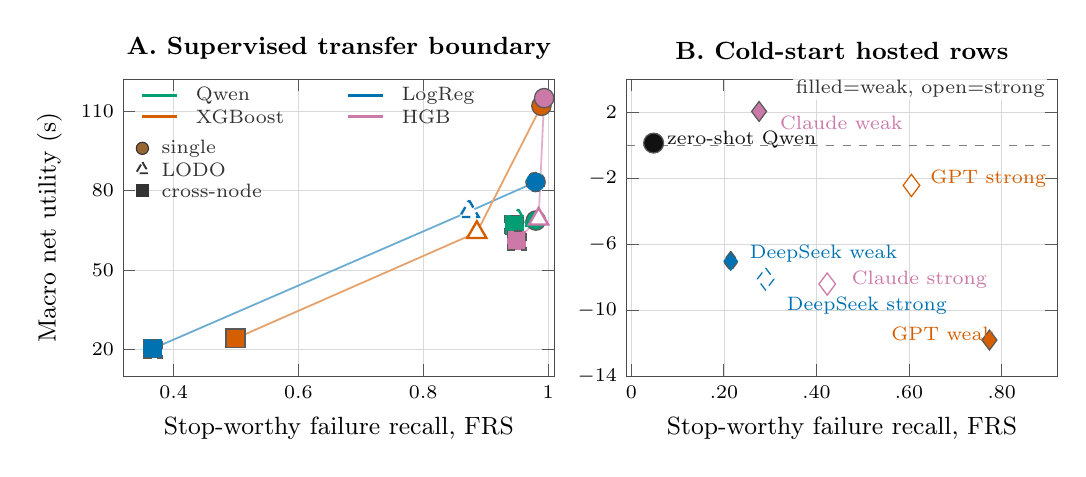
\begin{tikzpicture}
\begin{groupplot}[
  group style={group name=capbd, group size=2 by 1, horizontal sep=0.92cm},
  width=7.05cm,
  height=5.35cm,
  xlabel={Stop-worthy failure recall, FRS},
  ylabel={Macro net utility (s)},
  xlabel style={font=\small},
  ylabel style={font=\small},
  tick label style={font=\scriptsize},
  title style={font=\small\bfseries, yshift=-0.5ex},
  scaled ticks=false,
  axis line style={black!70, line width=0.35pt},
  tick style={black!65, line width=0.35pt},
  ymajorgrids,
  xmajorgrids,
  grid style={gridC, line width=0.25pt},
  clip marker paths=true,
]
\nextgroupplot[
  title={A. Supervised transfer boundary},
  xmin=0.32,
  xmax=1.01,
  ymin=10,
  ymax=122,
  xtick={0.4,0.6,0.8,1.0},
  ytick={20,50,80,110},
]
\addplot+[no marks, color=qwenC!58, line width=0.65pt] coordinates {(0.9805,68.75) (0.9522,68.82) (0.9458,67.12)};
\addplot+[no marks, color=logregC!58, line width=0.65pt] coordinates {(0.9800,83.27) (0.8737,72.18) (0.3667,20.40)};
\addplot+[no marks, color=xgbC!58, line width=0.65pt] coordinates {(0.9894,112.05) (0.8859,64.26) (0.4992,24.24)};
\addplot+[no marks, color=hgbC!58, line width=0.65pt] coordinates {(0.9938,114.95) (0.9849,69.33) (0.9496,61.22)};
\addplot+[only marks, mark=*, mark size=3.5pt, color=qwenC, fill=qwenC, mark options={line width=0.45pt, draw=black!65}] coordinates {(0.9805,68.75)};
\addplot+[only marks, mark=triangle*, mark size=4.0pt, color=qwenC, fill=white, mark options={line width=0.85pt, draw=qwenC}] coordinates {(0.9522,68.82)};
\addplot+[only marks, mark=square*, mark size=3.4pt, color=qwenC, fill=qwenC, mark options={line width=0.45pt, draw=black!65}] coordinates {(0.9458,67.12)};
\addplot+[only marks, mark=*, mark size=3.5pt, color=logregC, fill=logregC, mark options={line width=0.45pt, draw=black!65}] coordinates {(0.9800,83.27)};
\addplot+[only marks, mark=triangle*, mark size=4.0pt, color=logregC, fill=white, mark options={line width=0.85pt, draw=logregC}] coordinates {(0.8737,72.18)};
\addplot+[only marks, mark=square*, mark size=3.4pt, color=logregC, fill=logregC, mark options={line width=0.45pt, draw=black!65}] coordinates {(0.3667,20.40)};
\addplot+[only marks, mark=*, mark size=3.5pt, color=xgbC, fill=xgbC, mark options={line width=0.45pt, draw=black!65}] coordinates {(0.9894,112.05)};
\addplot+[only marks, mark=triangle*, mark size=4.0pt, color=xgbC, fill=white, mark options={line width=0.85pt, draw=xgbC}] coordinates {(0.8859,64.26)};
\addplot+[only marks, mark=square*, mark size=3.4pt, color=xgbC, fill=xgbC, mark options={line width=0.45pt, draw=black!65}] coordinates {(0.4992,24.24)};
\addplot+[only marks, mark=*, mark size=3.5pt, color=hgbC, fill=hgbC, mark options={line width=0.45pt, draw=black!65}] coordinates {(0.9938,114.95)};
\addplot+[only marks, mark=triangle*, mark size=4.0pt, color=hgbC, fill=white, mark options={line width=0.85pt, draw=hgbC}] coordinates {(0.9849,69.33)};
\addplot+[only marks, mark=square*, mark size=3.4pt, color=hgbC, fill=hgbC, mark options={line width=0.45pt, draw=black!65}] coordinates {(0.9496,61.22)};
\draw[qwenC, line width=0.9pt] (axis cs:0.35,116) -- (axis cs:0.405,116);
\node[font=\scriptsize, anchor=west, text=textC] at (axis cs:0.420,116) {Qwen};
\draw[logregC, line width=0.9pt] (axis cs:0.68,116) -- (axis cs:0.735,116);
\node[font=\scriptsize, anchor=west, text=textC] at (axis cs:0.750,116) {LogReg};
\draw[xgbC, line width=0.9pt] (axis cs:0.35,108) -- (axis cs:0.405,108);
\node[font=\scriptsize, anchor=west, text=textC] at (axis cs:0.420,108) {XGBoost};
\draw[hgbC, line width=0.9pt] (axis cs:0.68,108) -- (axis cs:0.735,108);
\node[font=\scriptsize, anchor=west, text=textC] at (axis cs:0.750,108) {HGB};
\addplot+[only marks, mark=*, mark size=2.2pt, color=textC, fill=textC] coordinates {(0.35,96)};
\addplot+[only marks, mark=triangle*, mark size=2.7pt, color=textC, fill=white, mark options={line width=0.70pt, draw=textC}] coordinates {(0.35,88)};
\addplot+[only marks, mark=square*, mark size=2.2pt, color=textC, fill=textC] coordinates {(0.35,80)};
\node[font=\scriptsize, anchor=west, text=textC] at (axis cs:0.365,96) {single};
\node[font=\scriptsize, anchor=west, text=textC] at (axis cs:0.365,88) {LODO};
\node[font=\scriptsize, anchor=west, text=textC] at (axis cs:0.365,80) {cross-node};
\nextgroupplot[
  title={B. Cold-start hosted rows},
  xmin=-0.010,
  xmax=0.92,
  ymin=-14,
  ymax=4.0,
  ylabel={},
  xtick={0,0.20,0.40,0.60,0.80},
  xticklabels={0,.20,.40,.60,.80},
  ytick={-14,-10,-6,-2,2},
]
\draw[dashed, black!50, line width=0.45pt] (axis cs:-0.010,0) -- (axis cs:0.92,0);
\addplot+[only marks, mark=*, mark size=3.6pt, color=zeroC, fill=zeroC, mark options={line width=0.45pt, draw=black!65}] coordinates {(0.0482,0.14)};
\node[font=\scriptsize, anchor=west, text=zeroC] at (axis cs:0.056,0.36) {zero-shot Qwen};
\addplot+[only marks, mark=diamond*, mark size=3.6pt, color=claudeC, fill=claudeC, mark options={line width=0.45pt, draw=black!65}] coordinates {(0.2759,2.06)};
\node[font=\scriptsize, anchor=west, text=claudeC] at (axis cs:0.300,1.38) {Claude weak};
\addplot+[only marks, mark=diamond*, mark size=4.0pt, color=claudeC, fill=white, mark options={line width=0.45pt, draw=claudeC}] coordinates {(0.4231,-8.41)};
\node[font=\scriptsize, anchor=west, text=claudeC] at (axis cs:0.455,-8.15) {Claude strong};
\addplot+[only marks, mark=diamond*, mark size=3.6pt, color=gptC, fill=gptC, mark options={line width=0.45pt, draw=black!65}] coordinates {(0.7736,-11.81)};
\node[font=\scriptsize, anchor=east, text=gptC] at (axis cs:0.805,-11.42) {GPT weak};
\addplot+[only marks, mark=diamond*, mark size=4.0pt, color=gptC, fill=white, mark options={line width=0.45pt, draw=gptC}] coordinates {(0.6051,-2.43)};
\node[font=\scriptsize, anchor=west, text=gptC] at (axis cs:0.625,-2.05) {GPT strong};
\addplot+[only marks, mark=diamond*, mark size=3.6pt, color=deepseekC, fill=deepseekC, mark options={line width=0.45pt, draw=black!65}] coordinates {(0.2147,-7.03)};
\node[font=\scriptsize, anchor=west, text=deepseekC] at (axis cs:0.235,-6.55) {DeepSeek weak};
\addplot+[only marks, mark=diamond*, mark size=4.0pt, color=deepseekC, fill=white, mark options={line width=0.45pt, draw=deepseekC}] coordinates {(0.2901,-8.11)};
\node[font=\scriptsize, anchor=west, text=deepseekC] at (axis cs:0.315,-9.75) {DeepSeek strong};
\node[font=\scriptsize, anchor=east, text=textC, fill=white, fill opacity=0.86, text opacity=1, inner sep=1pt] at (axis cs:0.90,3.45) {filled=weak, open=strong};
\end{groupplot}
\end{tikzpicture}
\end{document}
